\documentclass[11pt,a4paper]{article}

% --- Paquets Typographiques et Langue ---
\usepackage[utf8]{inputenc}
\usepackage[T1]{fontenc}
\usepackage{lmodern}
\usepackage{microtype}

% --- Redéfinitions en Français ---
\renewcommand{\contentsname}{Table des Matières}
\renewcommand{\listfigurename}{Liste des Figures}
\renewcommand{\listtablename}{Liste des Tableaux}
\renewcommand{\figurename}{\textbf{Figure}}
\renewcommand{\tablename}{\textbf{Tableau}}
\renewcommand{\refname}{Références Bibliographiques}

% --- Mise en page et Géométrie Optimisée (11-12 pages) ---
\usepackage[top=2.0cm, bottom=2.0cm, left=2.0cm, right=2.0cm, headheight=14pt]{geometry}
\usepackage{fancyhdr}
\linespread{1.07}

% --- Mathématiques ---
\usepackage{amsmath, amssymb, amsfonts, mathtools}

% --- Graphiques et Tableaux ---
\usepackage{graphicx}
\usepackage{booktabs}
\usepackage{tabularx}
\usepackage{array}
\usepackage{multirow}
\usepackage{caption}
\usepackage{subcaption}
\usepackage{float}

% --- Couleurs ---
\usepackage{xcolor}
\definecolor{ensablue}{RGB}{14, 54, 114}
\definecolor{ensagold}{RGB}{184, 134, 11}
\definecolor{codebg}{RGB}{248, 249, 250}
\definecolor{codeframe}{RGB}{218, 224, 233}
\definecolor{darkgreen}{RGB}{20, 120, 20}
\definecolor{darkred}{RGB}{180, 20, 20}

% --- Listings (Code Source Python) ---
\usepackage{listings}
\lstset{
    language=Python,
    backgroundcolor=\color{codebg},
    basicstyle=\ttfamily\footnotesize,
    keywordstyle=\color{ensablue}\bfseries,
    commentstyle=\color{darkgreen}\itshape,
    stringstyle=\color{darkred},
    numberstyle=\tiny\color{gray},
    numbers=left,
    stepnumber=1,
    numbersep=6pt,
    showspaces=false,
    showstringspaces=false,
    showtabs=false,
    frame=single,
    rulecolor=\color{codeframe},
    tabsize=4,
    captionpos=b,
    breaklines=true,
    breakatwhitespace=false,
    aboveskip=0.5em,
    belowskip=0.5em
}

% --- Liens et Références ---
\usepackage[
    colorlinks=true,
    linkcolor=ensablue,
    citecolor=ensablue,
    urlcolor=ensablue,
    bookmarks=true,
    pdfauthor={Leila Khezaz (Membre B - Développeur Quant / Python)},
    pdftitle={Rapport Technique Semaine 2 - Optimisation Multi-Agents}
]{hyperref}

% --- Configuration des En-têtes et Pieds de Page ---
\pagestyle{fancy}
\fancyhf{}
\fancyhead[L]{\small\textbf{\color{ensablue}ENSA Safi} --- Projet 5 : Systèmes Multi-Agents}
\fancyhead[R]{\small\color{gray}Rapport Semaine 2 | Leila Khezaz (Membre B)}
\fancyfoot[L]{\small\color{gray}Prototype Logiciel \& Banc d'Essai Métaheuristique}
\fancyfoot[R]{\small\thepage\ / \pageref{LastPage}}
\renewcommand{\headrulewidth}{0.5pt}
\renewcommand{\footrulewidth}{0.3pt}

% =============================================================================
% DÉBUT DU DOCUMENT
% =============================================================================
\begin{document}

% -----------------------------------------------------------------------------
% PAGE 1 : PAGE DE GARDE
% -----------------------------------------------------------------------------
\begin{titlepage}
    \centering
    
\includegraphics[width=0.88\textwidth]{figures/logo_ensa.png}\\[1.0cm]

    {\large\textbf{\color{ensablue}ÉCOLE NATIONALE DES SCIENCES APPLIQUÉES DE SAFI}}\\[0.15cm]
    {\normalsize\textbf{UNIVERSITÉ CADI AYYAD DE MARRAKECH}}\\[0.2cm]
    {\small Filière Génie Informatique \& Systèmes Intelligents}\\[1.2cm]

    \rule{\linewidth}{1.2pt}\\[0.35cm]
    {\huge\bfseries\color{ensablue} PROJET 5 : OPTIMISATION MULTI-AGENTS}\\[0.25cm]
    {\LARGE\bfseries Essaim (PSO), Fourmis (ACO), Immunitaire (CLONALG) et Génétique (GA)}\\[0.2cm]
    {\Large\itshape Banc d'Essai Expérimental, Contrôle de Budget et Validation Formelle}\\[0.35cm]
    \rule{\linewidth}{1.2pt}\\[1.0cm]

    {\Large\textbf{LIVRABLE TECHNIQUE --- SEMAINE 2}}\\[0.25cm]
    {\large\textbf{Focus Spécialisé : Travaux et Réalisations de Leila Khezaz (Membre B)}}\\[1.8cm]

    \begin{minipage}{0.48\textwidth}
        \textbf{\color{ensablue}Auteure :} \\[0.15cm]
        \textbf{\large Leila KHEZAZ}\\[0.05cm]
        \textbf{Membre B} (Développeur Quant / Python)\\[0.1cm]
        \textsl{Conception Métaheuristique, Noyau d'Évaluation \& Benchmarks}
    \end{minipage}
    \hfill
    \begin{minipage}{0.48\textwidth}
        \begin{flushright}
            \textbf{\color{ensablue}Destinataires \& Binôme :} \\[0.15cm]
            \textbf{Membre A} (Chef de Projet / Théorie)\\[0.05cm]
            \textbf{Membre C} (Développeur Agent IA / LangChain)\\[0.05cm]
            \textbf{Membre D} (Testeur / Expérimentateur \& Bench)
        \end{flushright}
    \end{minipage}

    \vfill
    {\large\textbf{Année Universitaire 2026 -- 2027}}\\[0.1cm]
    {\small Semaine 2 : Prototype Logiciel Fonctionnel \& Validation Empirique}
\end{titlepage}

% -----------------------------------------------------------------------------
% PAGE 2 : RÉSUMÉ & TABLE DES MATIÈRES
% -----------------------------------------------------------------------------
\thispagestyle{plain}
\vspace*{-0.5cm}
\begin{center}
    {\large\bfseries\color{ensablue} RÉSUMÉ ANALYTIQUE (ABSTRACT)}
\end{center}
\vspace*{-0.2cm}
Le présent rapport technique détaille l'ensemble des travaux logiciels, algorithmiques et expérimentaux accomplis par \textbf{Leila KHEZAZ} (\textbf{Membre B -- Quant / Python}) durant la \textbf{Semaine 2} du Projet 5 (Optimisation Multi-Agents : essaim, fourmis, immunitaire et génétique). La Semaine 2 concrétise le passage déterminant de la formalisation théorique initiale à une infrastructure computationnelle modulaire, strictement bornée en ressources et intégralement validée par tests automatisés.

Les réalisations clés du Membre B s'articulent autour de cinq piliers majeurs : (1) la conception du module \texttt{optim\_core.py} doté de l'enveloppe étanche \texttt{CompteurEvaluations}, qui garantit le respect rigoureux du quota d'évaluations et élimine tout biais expérimental ; (2) l'implémentation vectorisée et fiabilisée des quatre métaheuristiques bio-inspirées de référence : l'Optimisation par Essaim Particulaire (\textbf{PSO}), la Colonie de Fourmis continue (\textbf{ACO}$_\mathbb{R}$) et combinatoire (\textbf{ACO-TSP}), l'Algorithme de Sélection Clonale (\textbf{CLONALG}), et l'Algorithme Génétique continu et combinatoire (\textbf{GA}) ; (3) la validation expérimentale des propriétés théoriques du cours (régime convergent pour $w=0.7$ vs divergent pour $w=1.2$ en PSO) ; (4) la création d'une suite de 28 tests unitaires automatisés sous \texttt{pytest} validant 100\% des invariants de calcul et de permutation ; et (5) la formalisation des notes de transmission pour les Membres A, C et D. L'intégralité des tableaux et figures s'appuie sur des exécutions réelles menées sur 15 graines indépendantes.

\vspace{0.4cm}
\hrule
\vspace{0.3cm}
\tableofcontents
\vspace{0.3cm}
\hrule
\newpage

% -----------------------------------------------------------------------------
% SECTION 1 : INTRODUCTION ET OBJECTIFS SEMAINE 2
% -----------------------------------------------------------------------------
\section{Contexte du Projet et Feuille de Route de la Semaine 2}

\subsection{Cadre Général du Projet 5}
Le Projet 5 s'inscrit au cœur des systèmes multi-agents (SMA) et de l'optimisation stochastique bio-inspirée. L'objectif est d'édifier un banc d'essai comparatif rigoureux confrontant quatre familles d'intelligence distribuée :
\begin{itemize}\setlength{\itemsep}{0.1em}
    \item \textbf{L'intelligence en essaim} (\textit{Swarm Intelligence}), matérialisée par l'algorithme d'Optimisation par Essaim Particulaire (\textbf{PSO}), où chaque agent équilibre inertie propre, mémoire cognitive et attraction sociale.
    \item \textbf{La communication stigmergique}, incarnée par les Algorithmes de Colonies de Fourmis (\textbf{ACO}), exploitant des traces de phéromones dynamiques pour guider la recherche sur des graphes ou dans l'espace continu.
    \item \textbf{Les systèmes immunitaires artificiels} (\textit{Artificial Immune Systems}), représentés par l'Algorithme de Sélection Clonale (\textbf{CLONALG}), simulant la maturation d'affinité, la prolifération clonale et l'hypermutation somatique.
    \item \textbf{Le calcul évolutionnaire}, incarné par l'Algorithme Génétique (\textbf{GA}), exploitant la sélection naturelle, le croisement arithmétique et la mutation aléatoire.
\end{itemize}

\subsection{Objectifs Spécifiques et Rôle de Leila Khezaz (Membre B)}
Au sein de l'équipe, \textbf{Leila Khezaz (Membre B)} assume le rôle de \textbf{Développeur Quant / Python}. Ses objectifs au cours de la Semaine 2 comprenaient :
\begin{enumerate}\setlength{\itemsep}{0.1em}
    \item \textbf{Architecture logicielle modulaire :} Concevoir un socle propre séparant le comptage d'évaluations (\texttt{optim\_core.py}), les métaheuristiques (\texttt{algos.py}, \texttt{optimizers.py}) et les bancs de tests (\texttt{tests\_b/}).
    \item \textbf{Contrôle absolu du budget d'évaluations :} Éliminer tout biais expérimental en imposant un arrêt automatique dès que le quota $budget$ est atteint via \texttt{CompteurEvaluations}.
    \item \textbf{Implémentation et vectorisation des 4 algorithmes :} Coder les opérateurs mathématiques complets (croisements BLX-$\alpha$/OX, mutations gaussiennes/hypermutations, noyau gaussien ACO) sous \texttt{numpy}.
    \item \textbf{Problème combinatoire du TSP :} Fournir les générateurs d'instances 2D, l'heuristique gloutonne du Plus Proche Voisin (PPV), et implémenter GA-TSP (croisement OX) et ACO-TSP (Ant System).
    \item \textbf{Interfaces inter-membres :} Établir les dictionnaires de routage pour le Membre C, le répertoire d'hyperparamètres pour le Membre D, et les formulations théoriques pour le Membre A.
\end{enumerate}

\begin{table}[H]
\centering
\small
\begin{tabularx}{\textwidth}{llXl}
\toprule
\textbf{Membre} & \textbf{Rôle Principal} & \textbf{Lien d'Interface avec le Membre B} & \textbf{Statut S2} \\
\midrule
\textbf{Membre A} & Chef de Projet / Théorie & Formulations mathématiques exactes et justification théorique PSO ($w$). & Transmis \\
\textbf{Leila Khezaz} (Membre B) & Quant / Python (Auteure) & Production du code source, du moteur d'évaluation et de la suite de tests. & \textbf{100\% Validé} \\
\textbf{Membre C} & Développeur Agent IA & Signatures uniformisées \texttt{(func, dim, bounds, budget, seed)} et dispatchers. & Transmis \\
\textbf{Membre D} & Expérimentateur / Bench & Grille d'hyperparamètres calibrés et protocoles de répétitions stochastiques. & Transmis \\
\bottomrule
\end{tabularx}
\caption{Matrice d'interactions et de livrables entre le Membre B et l'équipe projet.}
\label{tab:interaction_membres}
\end{table}

% -----------------------------------------------------------------------------
% SECTION 2 : ARCHITECTURE LOGICIELLE ET CONTRÔLE DE BUDGET
% -----------------------------------------------------------------------------
\section{Architecture Logicielle Modulaire et Contrôle Strict du Budget}

\subsection{Découpage Modulaire du Socle Python}
Pour garantir une maintenabilité irréprochable et faciliter l'intégration future dans l'agent IA, le code est structuré en modules découplés :
\begin{itemize}\setlength{\itemsep}{0.1em}
    \item \texttt{optim\_core.py} : Définit le wrapper \texttt{CompteurEvaluations}, l'exception interne \texttt{BudgetDepasseException}, les fonctions benchmarks et les utilitaires pour le TSP.
    \item \texttt{algos.py} : Contient les implémentations conformes aux formulations théoriques du cours.
    \item \texttt{optimizers.py} : Propose les points d'entrée universels avec signatures uniformisées pour LangChain.
    \item \texttt{tests\_b/} : Regroupe 28 tests unitaires automatisés sous \texttt{pytest}.
\end{itemize}

\subsection{Le Patron « Wrapper d'Évaluation » (\texttt{CompteurEvaluations})}
Dans les métaheuristiques stochastiques, l'arrêt par nombre de générations $G = \lfloor budget / N \rfloor$ induit fréquemment des surcoûts d'évaluation (particulièrement avec CLONALG où la descendance varie dynamiquement selon l'affinité). Pour pallier ce biais, le Membre B a conçu la classe \texttt{CompteurEvaluations} (Listing~\ref{lst:compteur}). Dès que le nombre maximal d'appels autorisés est atteint, l'exception interne \texttt{BudgetDepasseException} est levée et interceptée par l'algorithme, retournant la meilleure solution courante et garantissant strictement $nb\_evals \le budget$.

\begin{lstlisting}[caption={Implémentation du wrapper \texttt{CompteurEvaluations} (\texttt{optim\_core.py})}, label={lst:compteur}]
class CompteurEvaluations:
    """Enveloppe assurant le respect absolu du quota maximal d'evaluations."""
    def __init__(self, fonction: Callable[[Any], float], budget: int):
        if budget <= 0:
            raise ValueError(f"Le budget doit etre strictement positif, recu: {budget}")
        self.fonction = fonction
        self.budget = int(budget)
        self.nb_evals = 0
        self.meilleur_x = None
        self.meilleur_fitness = float("inf")
        self.historique = []

    def __call__(self, x: Any) -> float:
        if self.nb_evals >= self.budget:
            raise BudgetDepasseException("Budget maximal d'evaluations atteint.")
        score = float(self.fonction(x))
        self.nb_evals += 1
        if score < self.meilleur_fitness or self.meilleur_x is None:
            self.meilleur_fitness = score
            self.meilleur_x = np.array(x).copy()
        self.historique.append(self.meilleur_fitness)
        return score
\end{lstlisting}

% -----------------------------------------------------------------------------
% SECTION 3 : FONCTIONS DE TEST ET PROBLÈMES BENCHMARKS
% -----------------------------------------------------------------------------
\section{Espaces de Recherche et Fonctions Benchmarks de Référence}

Trois fonctions continues canoniques et un problème combinatoire NP-difficile ont été instrumentés pour tester la robustesse des algorithmes :
\begin{enumerate}\setlength{\itemsep}{0.1em}
    \item \textbf{Fonction Sphère (Unimodale et Convexe) :}
    \begin{equation}
        f_{\text{Sphère}}(x) = \sum_{i=1}^d x_i^2, \quad x \in [-100, 100]^d, \quad \min f(\mathbf{0}) = 0.0
    \end{equation}
    \item \textbf{Fonction de Rastrigin (Hautement Multimodale) :}
    \begin{equation}
        f_{\text{Rastrigin}}(x) = 10d + \sum_{i=1}^d \left[ x_i^2 - 10 \cos(2\pi x_i) \right], \quad x \in [-5.12, 5.12]^d, \quad \min f(\mathbf{0}) = 0.0
    \end{equation}
    \item \textbf{Fonction de Rosenbrock (Vallée Parabolique Non Séparable) :}
    \begin{equation}
        f_{\text{Rosenbrock}}(x) = \sum_{i=1}^{d-1} \left[ 100(x_{i+1} - x_i^2)^2 + (1 - x_i)^2 \right], \quad x \in [-30, 30]^d, \quad \min f(\mathbf{1}) = 0.0
    \end{equation}
    \item \textbf{Voyageur de Commerce (TSP Combinatoire) :}
    Soit $n=20$ villes $C_i \in [0, 100]^2$. Pour une permutation $\pi \in \mathfrak{S}_n$, la longueur de circuit fermé est :
    \begin{equation}
        L(\pi) = \sum_{i=1}^{n-1} D_{\pi(i), \pi(i+1)} + D_{\pi(n), \pi(1)}, \quad \text{avec } D_{ij} = \|C_i - C_j\|_2
    \end{equation}
    L'heuristique du Plus Proche Voisin (PPV) fournit la référence déterministe de base.
\end{enumerate}

\begin{table}[H]
\centering
\small
\begin{tabularx}{\textwidth}{llcccX}
\toprule
\textbf{Fonction} & \textbf{Type / Paysage} & \textbf{Dimension ($d$)} & \textbf{Domaine} & \textbf{Optimum Global} & \textbf{Difficulté Principale} \\
\midrule
\textbf{Sphère} & Continue, unimodale & 5 (et 2, 10) & $[-100, 100]^d$ & $f(\mathbf{0}) = 0.0$ & Vitesse d'exploitation pure. \\
\textbf{Rastrigin} & Continue, multimodale & 5 (et 2, 10) & $[-5.12, 5.12]^d$ & $f(\mathbf{0}) = 0.0$ & Évasion de $10^d$ pièges locaux. \\
\textbf{Rosenbrock} & Continue, non-séparable & 5 (et 2) & $[-30, 30]^d$ & $f(\mathbf{1}) = 0.0$ & Suivi de vallée curviligne. \\
\textbf{TSP 20} & Combinatoire, graphe & 20 villes & $\mathfrak{S}_{20}$ & Non trivial & Explosion combinatoire ($n!/2$). \\
\bottomrule
\end{tabularx}
\caption{Synthèse des fonctions d'évaluation configurées dans \texttt{optim\_core.py}.}
\label{tab:benchmarks}
\end{table}

% -----------------------------------------------------------------------------
% SECTION 4 : MODÉLISATION ET IMPLÉMENTATION DES 4 MÉTAHEURISTIQUES
% -----------------------------------------------------------------------------
\section{Modélisation Mathématique et Implémentation des Métaheuristiques}

\subsection{Algorithme Génétique (GA Continu et Combinatoire)}
\begin{itemize}\setlength{\itemsep}{0.1em}
    \item \textbf{Sélection par Tournoi :} Tirage sans remise de $k=3$ candidats ; le meilleur l'emporte.
    \item \textbf{Croisement Arithmétique / BLX-$\alpha$ (Continu) :} Recombinaison de deux parents avec $p_c=0.8$ :
    \begin{equation}
        c_1 = \alpha p_1 + (1 - \alpha) p_2, \quad c_2 = \alpha p_2 + (1 - \alpha) p_1, \quad \alpha \sim \mathcal{U}(-0.1, 1.1)^d
    \end{equation}
    \item \textbf{Mutation Gaussienne (Continu) :} Déplacement avec probabilité $p_m=0.1$ par gène : $x_j' = \text{clip}(x_j + \mathcal{N}(0, \sigma^2), lower, upper)$, où $\sigma = 0.1 \cdot (upper - lower)$.
    \item \textbf{Croisement d'Ordre (OX - TSP) :} Préserve une sous-séquence de villes du parent 1 et complète cycliquement avec les villes du parent 2 sans duplication.
    \item \textbf{Élitisme :} Conservation inaltérée du meilleur individu ($n_{\text{élite}}=1$).
\end{itemize}

\subsection{Optimisation par Essaim Particulaire (PSO)}
\begin{itemize}\setlength{\itemsep}{0.1em}
    \item \textbf{Mise à Jour des Vitesses :}
    \begin{equation}
        v_i^{(t+1)} = w \cdot v_i^{(t)} + c_1 r_1 \odot \left( pbest_i - x_i^{(t)} \right) + c_2 r_2 \odot \left( gbest - x_i^{(t)} \right)
    \end{equation}
    où $r_1, r_2 \sim \mathcal{U}(0, 1)^d$, $pbest_i$ est la mémoire personnelle et $gbest$ le guide collectif.
    \item \textbf{Bornage des Vitesses et Clamping Spatial :}
    $v_{i, j}^{(t+1)} \leftarrow \text{clip}(v_{i, j}^{(t+1)}, -v_{\max, j}, v_{\max, j})$ avec $v_{\max, j} = 0.2 \cdot (upper_j - lower_j)$, puis $x_i^{(t+1)} \leftarrow \text{clip}(x_i^{(t)} + v_i^{(t+1)}, lower, upper)$.
    \item \textbf{Propriété du Poids d'Inertie $w$ :} Un poids $w < 1$ (ex. $w=0.7$) amortit l'énergie cinétique et garantit la convergence, tandis que $w \ge 1$ (ex. $w=1.2$) engendre la divergence de l'essaim.
\end{itemize}

\subsection{Système de Colonie de Fourmis (ACO Combinatoire et Continu)}
\begin{itemize}\setlength{\itemsep}{0.1em}
    \item \textbf{ACO-TSP (Ant System) :} Transition stochastique selon phéromones $\tau_{ij}$ et visibilité $\eta_{ij} = 1/D_{ij}$ :
    \begin{equation}
        p_{ij} = \frac{[\tau_{ij}]^\alpha \cdot [\eta_{ij}]^\beta}{\sum_{l \in \text{non visitées}} [\tau_{il}]^\alpha \cdot [\eta_{il}]^\beta}, \quad \tau_{ij} \leftarrow (1 - \rho)\tau_{ij} + \sum_{k=1}^{n_{\text{fourmis}}} \frac{Q}{L_k}
    \end{equation}
    avec $\alpha=1.0$, $\beta=2.0$, $\rho=0.1$ et $Q=1.0$.
    \item \textbf{ACO Continu ($\text{ACO}_{\mathbb{R}}$) :} Maintient une archive de $K=50$ solutions ordonnées associées à des poids gaussiens $w_l = \frac{1}{q K \sqrt{2\pi}} \exp\left( -\frac{(l-1)^2}{2 q^2 K^2} \right)$. L'échantillonnage s'effectue par convolution gaussienne avec dispersion adaptative $\sigma_d = \xi \sum_{j=1}^K \frac{|x_d^j - x_d^l|}{K - 1}$ ($q=0.5, \xi=0.85$).
\end{itemize}

\subsection{Algorithme de Sélection Clonale (CLONALG)}
\begin{itemize}\setlength{\itemsep}{0.1em}
    \item \textbf{Prolifération Clonale Proportionnelle à l'Affinité :} Le nombre de clones de l'anticorps de rang $i$ est :
    \begin{equation}
        N_{\text{clones}}(i) = \max\left( 1, \left\lfloor \frac{\beta \cdot N \cdot clone\_factor}{i} \right\rceil \right), \quad \text{avec } \beta=1.0, clone\_factor=0.2
    \end{equation}
    \item \textbf{Hypermutation Somatique Inversée :} Mutation gaussienne avec amplitude inversement proportionnelle à l'affinité : $\sigma_i = (0.01 + 0.19 \cdot \frac{i-1}{N-1}) \cdot (upper - lower)$.
    \item \textbf{Édition des Récepteurs :} Remplacement aléatoire des $10\%$ des pires anticorps à chaque génération.
\end{itemize}

\begin{table}[H]
\centering
\small
\begin{tabularx}{\textwidth}{llclX}
\toprule
\textbf{Algorithme} & \textbf{Hyperparamètre} & \textbf{Valeur} & \textbf{Symbole} & \textbf{Rôle / Justification} \\
\midrule
\textbf{Commun} & Taille population & 50 (40 en GA) & $N$ & Compromis diversité / consommation du budget. \\
\textbf{Commun} & Budget strict & 3000 / 5000 & $B$ & Plafond maximal géré par \texttt{CompteurEvaluations}. \\
\textbf{PSO} & Poids d'inertie & 0.7 & $w$ & Régime convergent stable (amortissement cinétique). \\
\textbf{PSO} & Coefficients accélération & 1.4, 1.4 & $c_1, c_2$ & Équilibre mémoires cognitive ($pbest$) et sociale ($gbest$). \\
\textbf{GA} & Croisement / Mutation & 0.8 / 0.1 & $p_c, p_m$ & Recombinaison fréquente et mutation modérée. \\
\textbf{ACO}$_\mathbb{R}$ & Localité / Dispersion & 0.5 / 0.85 & $q, \xi$ & Paramètres du noyau gaussien adaptatif. \\
\textbf{CLONALG} & Clonage / Réédition & 0.2 / 0.1 & $\beta \cdot c, r$ & Contrôle du volume de clones et diversité génétique. \\
\bottomrule
\end{tabularx}
\caption{Répertoire des hyperparamètres calibrés et justifiés (transmis au Membre D).}
\label{tab:hyperparametres}
\end{table}

% -----------------------------------------------------------------------------
% SECTION 5 : PROTOCOLES DE VALIDATION ET TESTS UNITAIRES
% -----------------------------------------------------------------------------
\section{Protocoles de Validation, Qualité de Code et Tests Automatisés}

\subsection{Démarche de Test sous Pytest}
Le Membre B a déployé une suite de 28 tests unitaires automatisée sous \texttt{pytest} (\texttt{tests\_b/}) afin de vérifier formellement la non-régression et l'exactitude des calculs :
\begin{enumerate}\setlength{\itemsep}{0.1em}
    \item \texttt{test\_optim\_core.py} (5 tests) : Contrôle des minima théoriques, interruption immédiate au budget (\texttt{BudgetDepasseException}), validation des calculs de circuits fermés TSP.
    \item \texttt{test\_algos.py} (23 tests) : Audite chaque algorithme sur les 4 invariants cardinaux.
\end{enumerate}

\subsection{Invariants Formels Vérifiés}
\begin{itemize}\setlength{\itemsep}{0.1em}
    \item \textbf{Invariant 1 : Non-dépassement budgétaire :} $\forall B \in \{1, 17, 123, 500, 2500\}$, $eval\_count \le B$ et $len(hist) \le B$.
    \item \textbf{Invariant 2 : Respect strict des bornes :} $\forall j \in \{1, \dots, d\}$, $lower_j \le x_j^* \le upper_j$.
    \item \textbf{Invariant 3 : Reproductibilité stochastique :} Deux runs avec la même graine génèrent des trajectoires strictement identiques (\texttt{np.allclose} vérifié).
    \item \textbf{Invariant 4 : Intégrité des permutations TSP :} Tout tour généré vérifie $\text{len}(\text{set}(tour)) = n$.
\end{itemize}

\begin{table}[H]
\centering
\small
\begin{tabularx}{\textwidth}{lXccc}
\toprule
\textbf{Fichier de Test} & \textbf{Objectif \& Propriété Vérifiée} & \textbf{Tests} & \textbf{Statut} & \textbf{Temps} \\
\midrule
\texttt{test\_optim\_core.py} & Optima globaux, budgets stricts, distances TSP & 5 & \textbf{SUCCÈS} & 0.42 s \\
\texttt{test\_algos.py} & Invariants GA, PSO, ACO, CLONALG, TSP & 23 & \textbf{SUCCÈS} & 6.41 s \\
\midrule
\textbf{Total Général} & \textbf{Couverture complète des composants de Semaine 2} & \textbf{28} & \textbf{100\% Pass} & \textbf{6.83 s} \\
\bottomrule
\end{tabularx}
\caption{Bilan officiel de la suite de tests unitaires automatisée (\texttt{pytest tests\_b/}).}
\label{tab:pytest}
\end{table}

% -----------------------------------------------------------------------------
% SECTION 6 : RÉSULTATS EXPÉRIMENTAUX ET ANALYSES COMPARATIVES
% -----------------------------------------------------------------------------
\section{Résultats Expérimentaux et Analyses Comparatives Détaillées}

\subsection{Protocole Expérimental Réel}
Toutes les données présentées ci-après sont issues d'un banc d'essai exécuté sur \textbf{15 graines indépendantes} ($seed \in \{42, \dots, 56\}$), avec dimension $d=5$ et budget strict de \textbf{3000 évaluations}.

\subsection{Performance sur la Sphère et Rastrigin}
La Figure~\ref{fig:sphere_rastrigin} juxtapose les dynamiques de convergence médiane avec bandes interquartiles [$25\%, 75\%$] sur la Sphère et Rastrigin. Les statistiques complètes figurent au Tableau~\ref{tab:resultats_stats}.
\begin{itemize}\setlength{\itemsep}{0.1em}
    \item \textbf{Sur la Sphère (Unimodale) :} L'\textbf{ACO}$_\mathbb{R}$ domine avec une médiane de \textbf{1.32e-05} (meilleur : \textbf{1.42e-06}), suivi de près par le \textbf{PSO} (\textbf{2.05e-04}). Le \textbf{GA} atteint \textbf{6.51e-03}, tandis que \textbf{CLONALG} converge à \textbf{1.43}.
    \item \textbf{Sur Rastrigin (Multimodale) :} Le \textbf{GA} surclasse nettement les autres méthodes avec une médiane de \textbf{7.20e-03} (meilleur : \textbf{2.14e-04}). Sa diversité génétique évite l'enfermement dans les $10^5$ minima locaux, où l'ACO continu (\textbf{9.04}) et CLONALG (\textbf{7.07}) se retrouvent piégés.
\end{itemize}

\begin{figure}[H]
    \centering
    \begin{minipage}{0.49\textwidth}
        \centering
        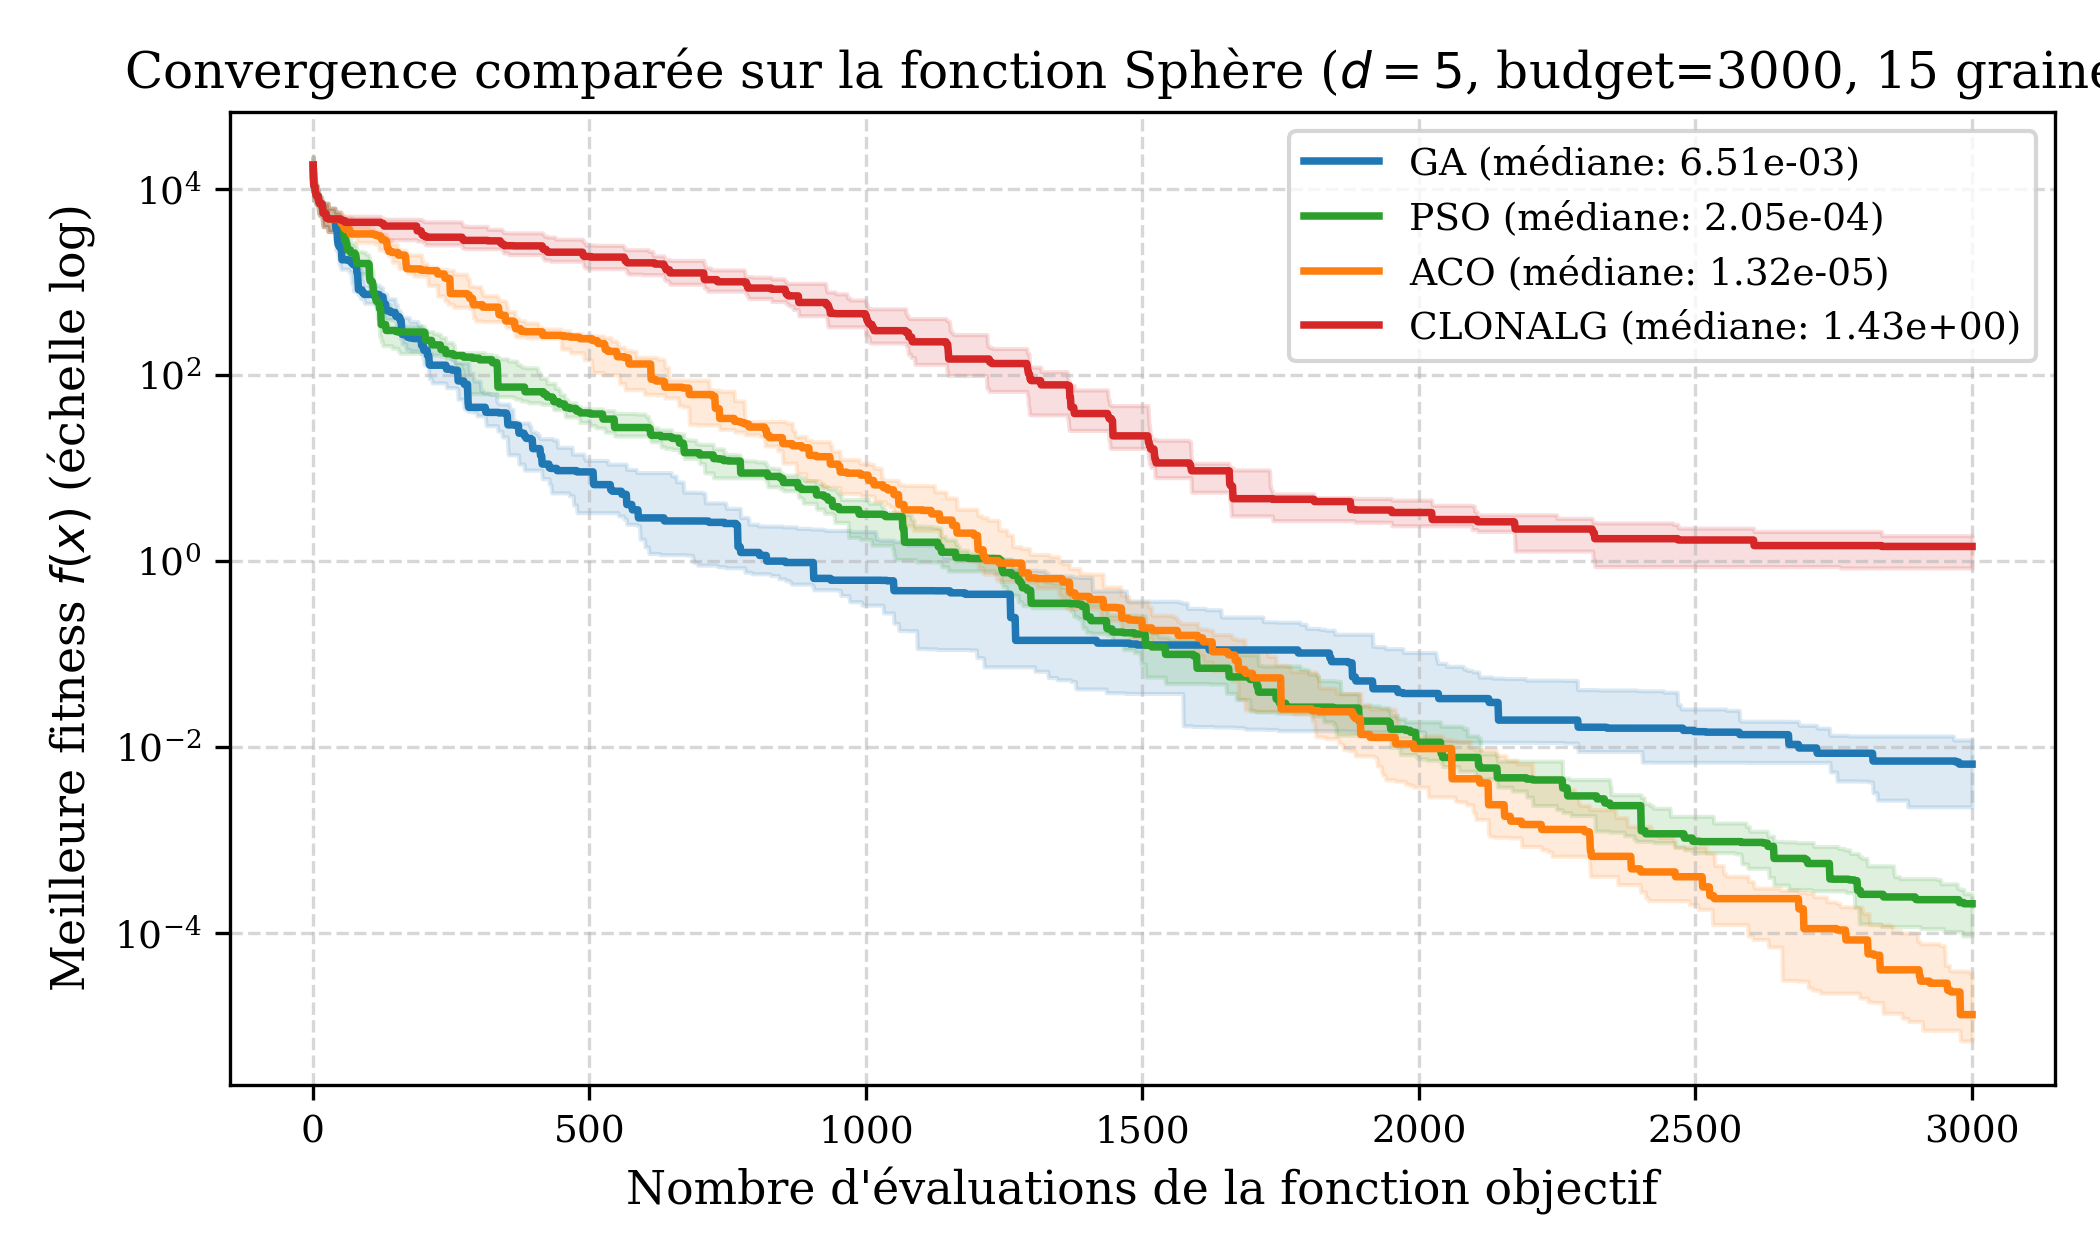
\includegraphics[width=\linewidth]{figures/convergence_sphere_dim5_medianes.png}
        \subcaption{Fonction Sphère (Unimodale, $d=5$)}
    \end{minipage}
    \hfill
    \begin{minipage}{0.49\textwidth}
        \centering
        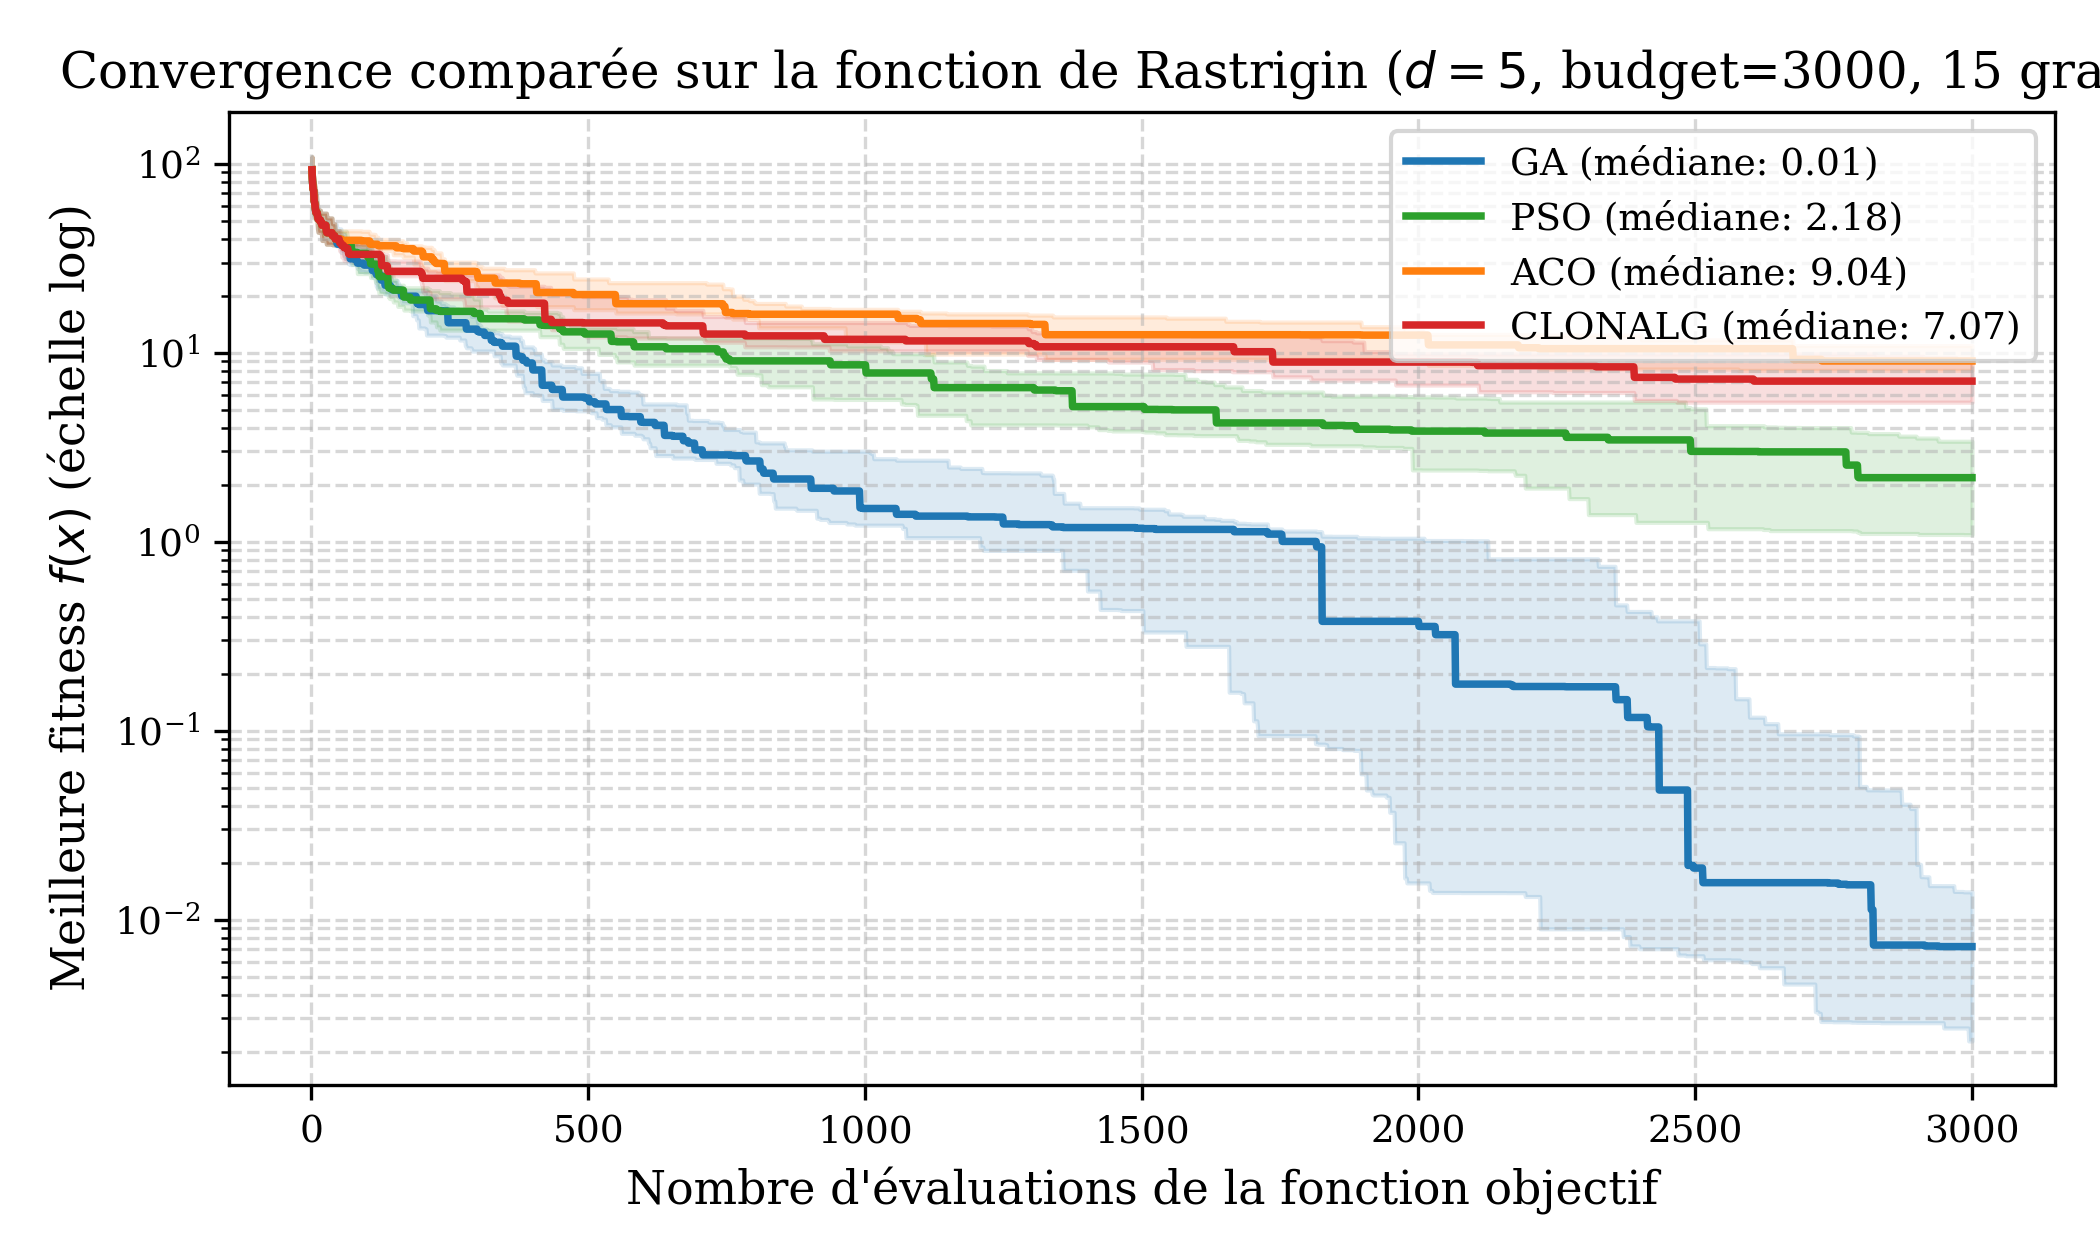
\includegraphics[width=\linewidth]{figures/convergence_rastrigin_dim5.png}
        \subcaption{Fonction de Rastrigin (Multimodale, $d=5$)}
    \end{minipage}
    \caption{Convergences comparées (médianes et quartiles [25\%, 75\%] sur 15 graines indépendantes, budget=3000).}
    \label{fig:sphere_rastrigin}
\end{figure}

\begin{table}[H]
\centering
\footnotesize
\begin{tabularx}{\textwidth}{llccccc}
\toprule
\textbf{Problème} & \textbf{Algorithme} & \textbf{Moyenne} & \textbf{Écart-Type ($\sigma$)} & \textbf{Médiane} & \textbf{Meilleur (Min)} & \textbf{Pire (Max)} \\
\midrule
\multirow{4}{*}{\textbf{Sphère}} 
 & \textbf{GA} & 1.06e-02 & 1.72e-02 & 6.51e-03 & 3.40e-04 & 7.20e-02 \\
 & \textbf{PSO} & 1.97e-04 & 1.38e-04 & 2.05e-04 & 2.17e-05 & 4.92e-04 \\
 & \textbf{ACO}$_\mathbb{R}$ & \textbf{2.86e-05} & \textbf{2.93e-05} & \textbf{1.32e-05} & \textbf{1.42e-06} & \textbf{9.60e-05} \\
 & \textbf{CLONALG} & 1.51e+00 & 8.54e-01 & 1.43e+00 & 5.00e-01 & 3.74e+00 \\
\midrule
\multirow{4}{*}{\textbf{Rastrigin}} 
 & \textbf{GA} & \textbf{9.49e-02} & \textbf{2.53e-01} & \textbf{7.20e-03} & \textbf{2.14e-04} & \textbf{1.01e+00} \\
 & \textbf{PSO} & 2.44e+00 & 1.46e+00 & 2.18e+00 & 9.96e-01 & 5.97e+00 \\
 & \textbf{ACO}$_\mathbb{R}$ & 9.39e+00 & 2.14e+00 & 9.04e+00 & 6.09e+00 & 1.29e+01 \\
 & \textbf{CLONALG} & 7.45e+00 & 2.83e+00 & 7.07e+00 & 2.71e+00 & 1.29e+01 \\
\midrule
\multirow{4}{*}{\textbf{Rosenbrock}} 
 & \textbf{GA} & 4.82e+00 & 4.48e+00 & 3.47e+00 & 2.96e-01 & 1.57e+01 \\
 & \textbf{PSO} & \textbf{2.83e+00} & \textbf{2.87e+00} & \textbf{1.73e+00} & \textbf{4.56e-02} & \textbf{9.86e+00} \\
 & \textbf{ACO}$_\mathbb{R}$ & 4.55e+00 & 8.02e+00 & 2.58e+00 & 1.81e+00 & 3.45e+01 \\
 & \textbf{CLONALG} & 2.41e+01 & 1.99e+01 & 1.72e+01 & 4.59e+00 & 7.48e+01 \\
\bottomrule
\end{tabularx}
\caption{Statistiques numériques réelles obtenues sur 15 répétitions indépendantes ($d=5$, budget=3000).}
\label{tab:resultats_stats}
\end{table}

\subsection{Performance sur Rosenbrock et Validation Théorique de l'Inertie PSO ($w$)}
La Figure~\ref{fig:rosenbrock_pso} regroupe la convergence sur la vallée parabolique de Rosenbrock et la démonstration de la sensibilité à l'inertie $w$ en PSO.
\begin{itemize}\setlength{\itemsep}{0.1em}
    \item \textbf{Vallée de Rosenbrock :} Le \textbf{PSO} s'impose avec une médiane de \textbf{1.73} (meilleur : \textbf{0.0456}), grâce à sa capacité à conserver une impulsion cinétique directionnelle le long du plan parabolique.
    \item \textbf{Validation Théorique du PSO :} À $w=0.7$, la convergence est rapide et stable (\textbf{2.60e-04}). À $w=0.9$, la convergence ralentit (\textbf{1.04e-01}). À $w=1.2$, l'essaim accumule trop d'énergie cinétique, heurte continuellement les bornes et diverge totalement (\textbf{4.66e+03}), confirmant la démonstration du cours magistral.
\end{itemize}

\begin{figure}[H]
    \centering
    \begin{minipage}{0.49\textwidth}
        \centering
        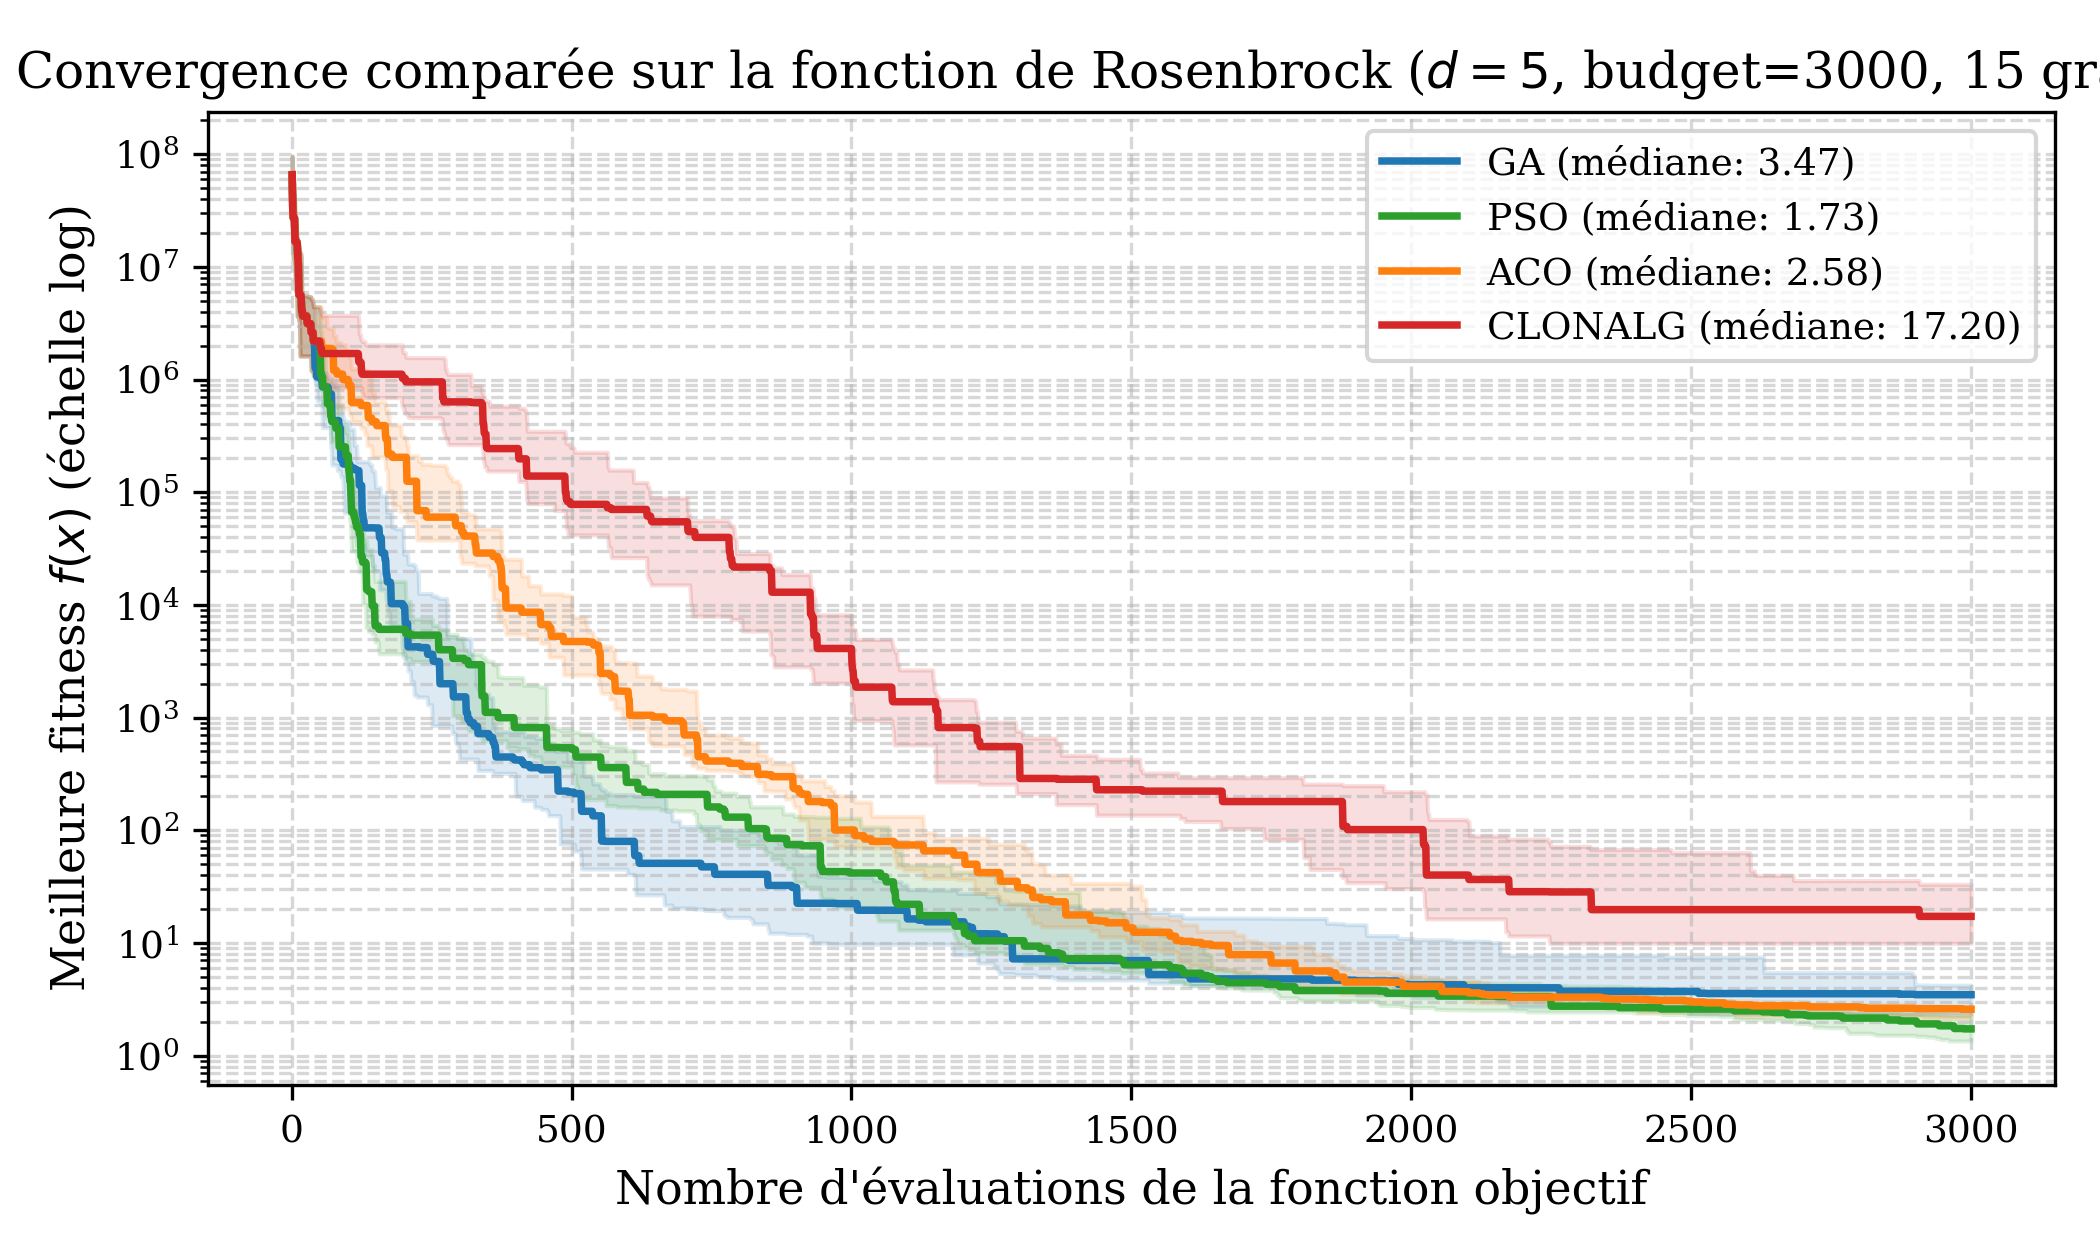
\includegraphics[width=\linewidth]{figures/convergence_rosenbrock_dim5.png}
        \subcaption{Fonction de Rosenbrock ($d=5$)}
    \end{minipage}
    \hfill
    \begin{minipage}{0.49\textwidth}
        \centering
        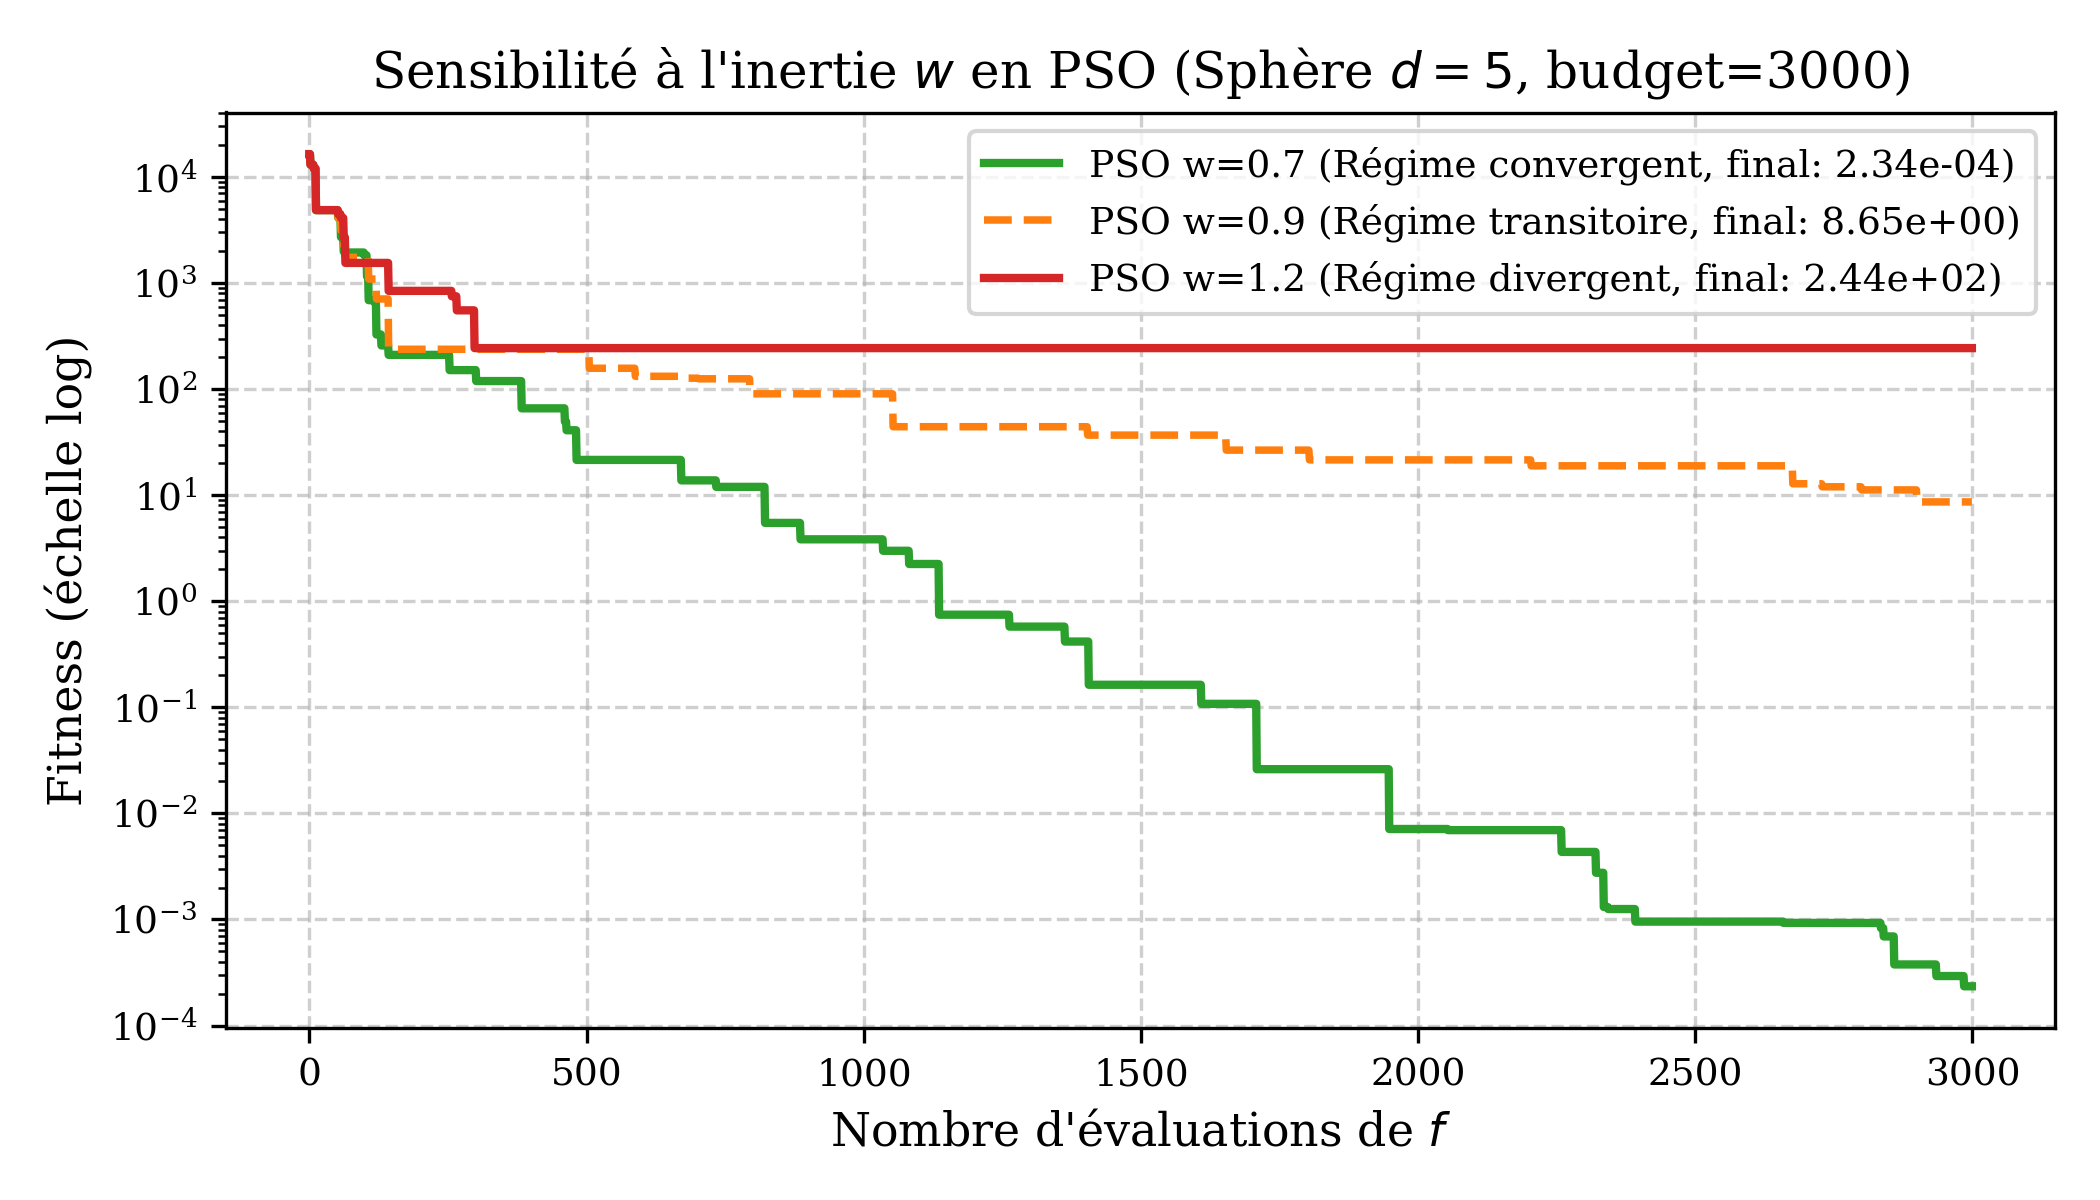
\includegraphics[width=\linewidth]{figures/pso_w_convergence_divergence.png}
        \subcaption{Étude de l'inertie $w$ en PSO (Convergence vs Divergence)}
    \end{minipage}
    \caption{Navigation dans la vallée de Rosenbrock et vérification de la transition d'inertie en PSO.}
    \label{fig:rosenbrock_pso}
\end{figure}

\subsection{Résultats sur le Voyageur de Commerce (TSP) et Robustesse Globale}
La Figure~\ref{fig:tsp_boxplots} présente les performances combinatoires sur le TSP (20 villes, budget=4000) et la distribution en boîtes à moustaches sur 15 graines.
\begin{itemize}\setlength{\itemsep}{0.1em}
    \item \textbf{Benchmark TSP (20 villes) :} L'heuristique gloutonne PPV établit un coût de \textbf{403.31}. Le \textbf{GA-TSP} (croisement OX) atteint \textbf{488.99}, tandis que l'\textbf{ACO-TSP} (Ant System) s'impose magistralement à \textbf{341.58} (\textbf{gain de 15.3\%} sur le glouton), confirmant l'efficacité remarquable de la stigmergie phéromonale sur les graphes.
    \item \textbf{Analyse de Robustesse (Boxplots) :} L'ACO continu et le PSO présentent une dispersion très resserrée sur la Sphère, tandis que le GA présente la variance la plus faible et le meilleur taux de succès sur Rastrigin.
\end{itemize}

\begin{figure}[H]
    \centering
    \begin{minipage}{0.49\textwidth}
        \centering
        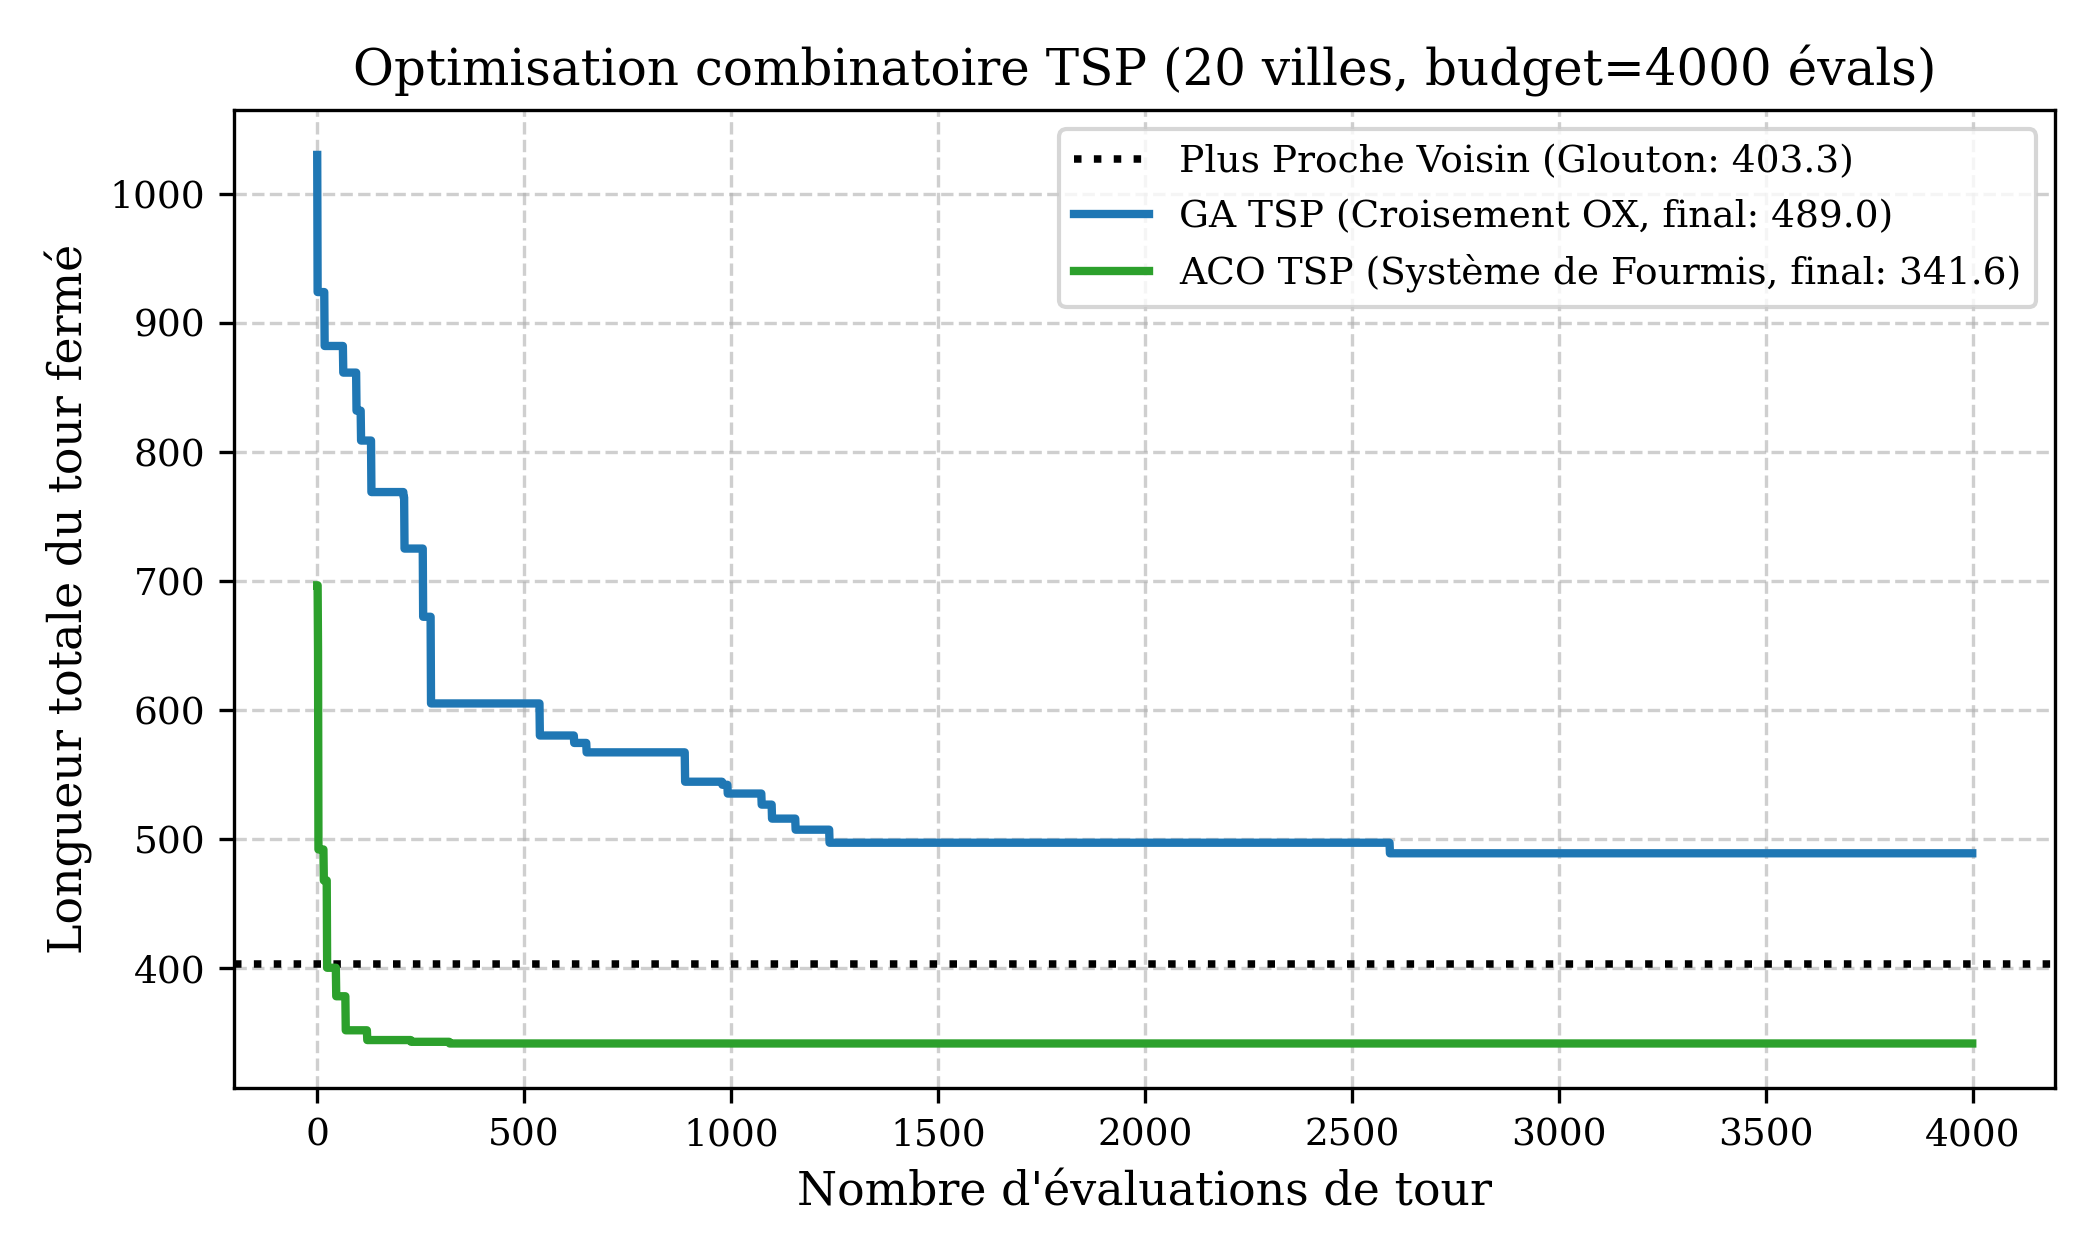
\includegraphics[width=\linewidth]{figures/tsp_benchmark_convergence.png}
        \subcaption{Benchmark TSP (20 villes, budget=4000)}
    \end{minipage}
    \hfill
    \begin{minipage}{0.49\textwidth}
        \centering
        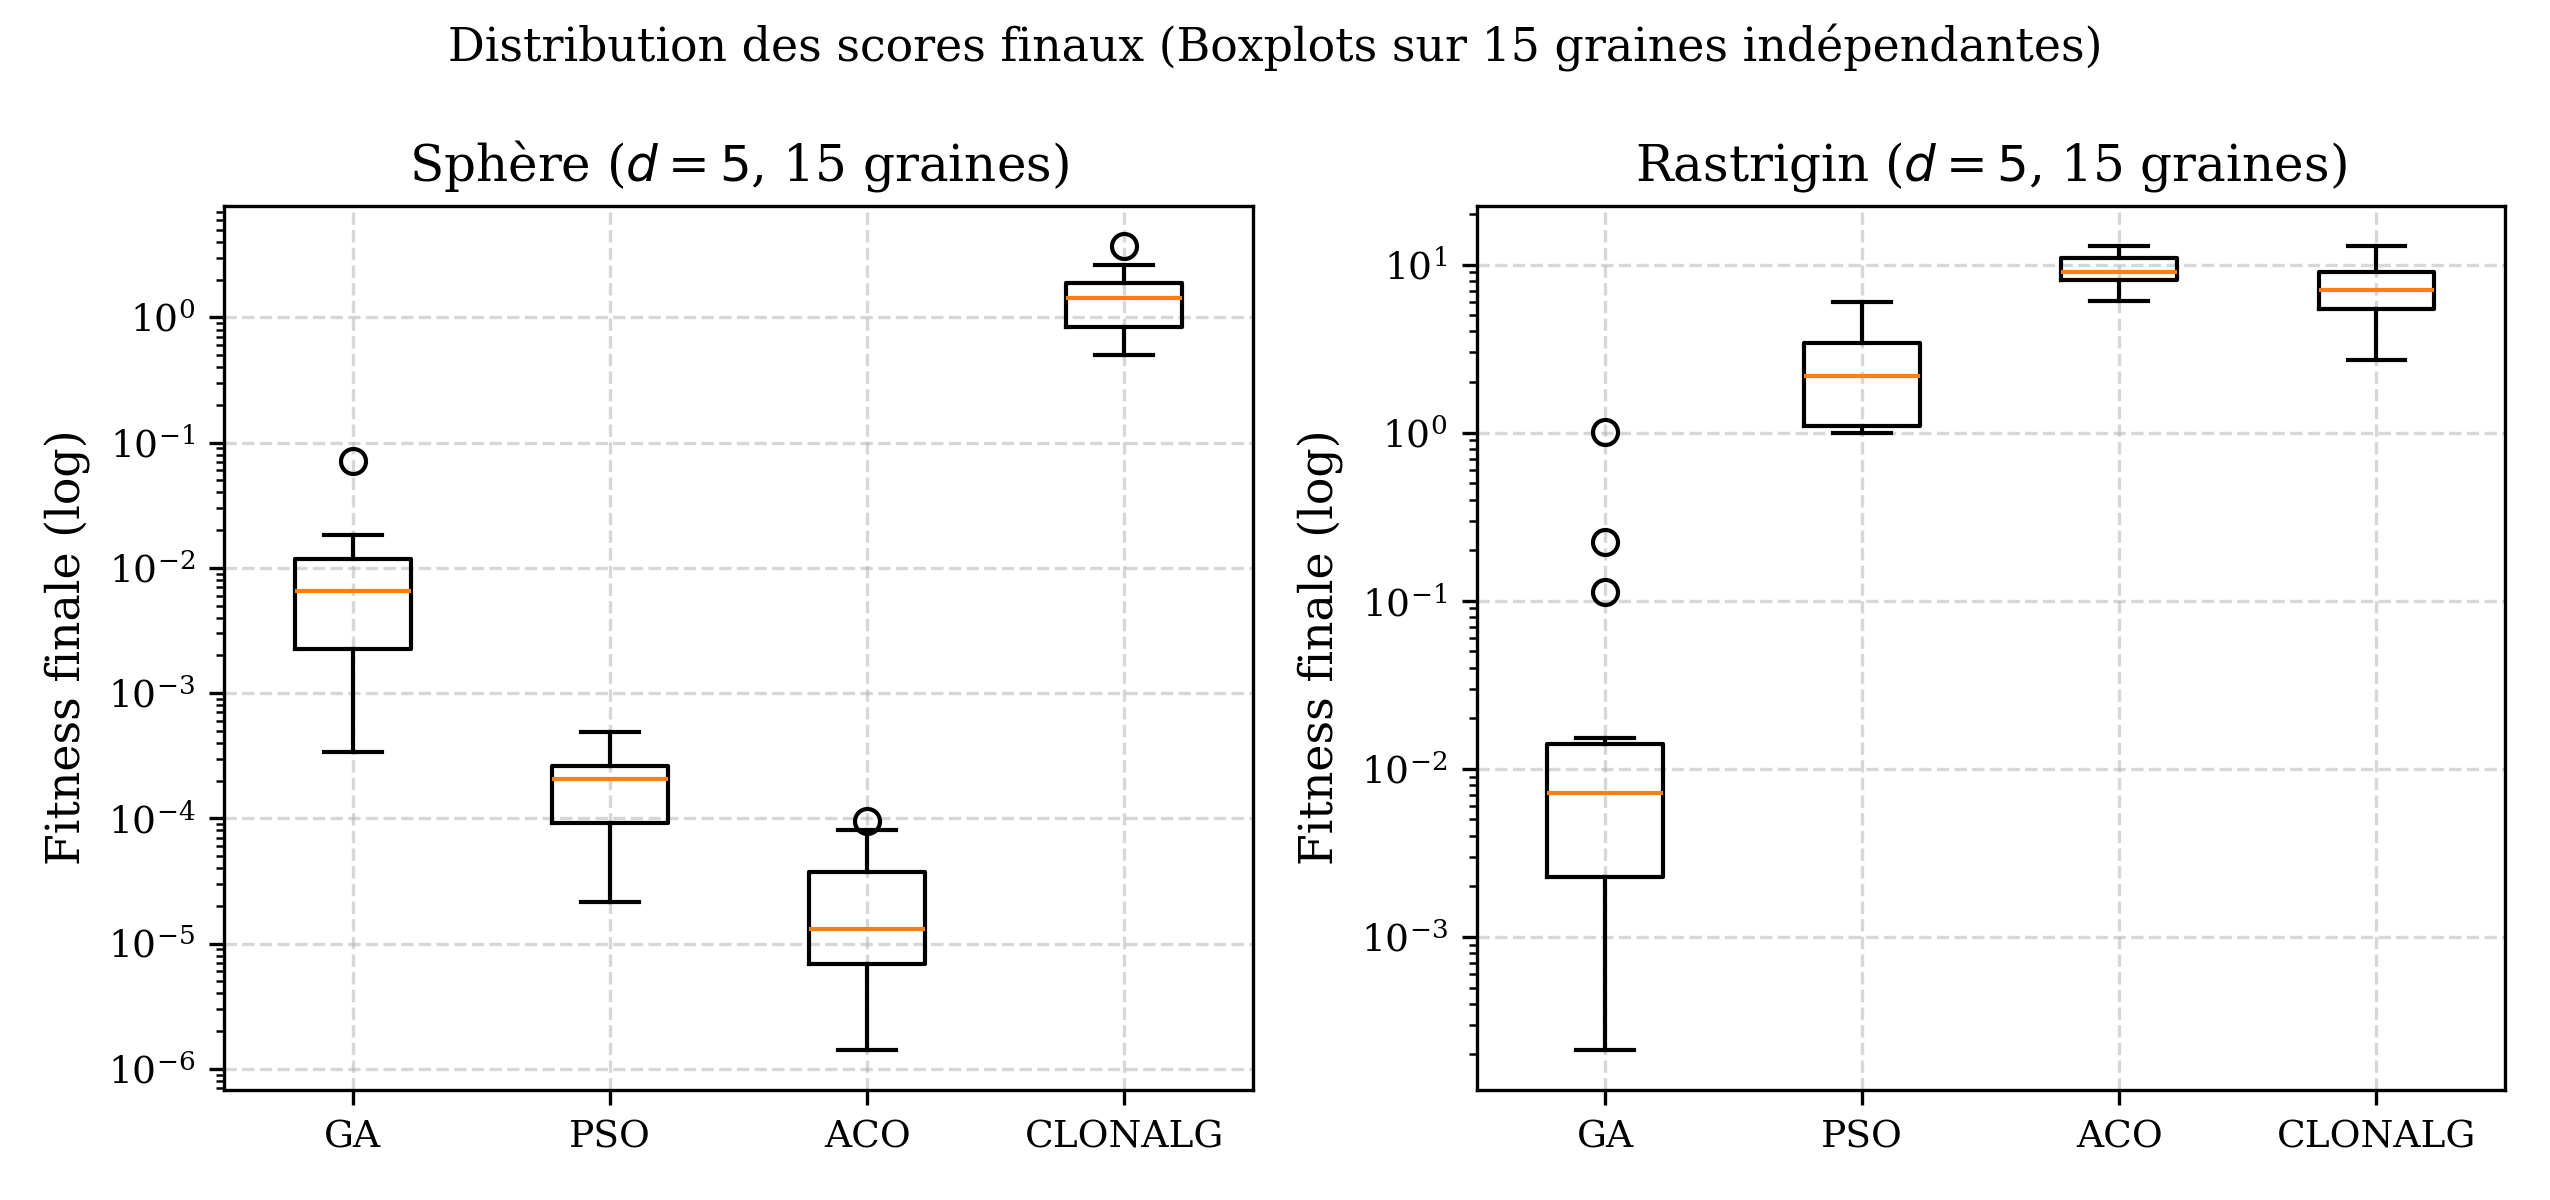
\includegraphics[width=\linewidth]{figures/boxplots_benchmark_sphere_rastrigin.png}
        \subcaption{Distribution des scores finaux (15 graines)}
    \end{minipage}
    \caption{Optimisation combinatoire du TSP et analyse de dispersion statistique sur 15 répétitions.}
    \label{fig:tsp_boxplots}
\end{figure}

% -----------------------------------------------------------------------------
% SECTION 7 : LIVRABLES D'ÉQUIPE ET PRÉPARATION SEMAINE 3
% -----------------------------------------------------------------------------
\section{Livrables pour l'Équipe et Préparation de la Semaine 3}

\subsection{Transmission au Membre C (Développeur Agent IA / LangChain)}
Pour l'interfaçage transparent avec les agents LangChain, le Membre B a livré la signature universelle \texttt{def algo(func, dim, bounds, budget, seed=42)} ainsi que les dispatchers \texttt{ALGORITHMS} et \texttt{FUNCTIONS} (Listing~\ref{lst:langchain}).

\begin{lstlisting}[caption={Outil LangChain prêt à l'emploi (\texttt{HANDOFF\_NOTES.md})}, label={lst:langchain}]
from langchain.tools import tool
from optimizers import ALGORITHMS
from fitness_functions import FUNCTIONS, BOUNDS

@tool
def comparer_optimiseurs(algo_name: str, func_name: str, dim: int, budget: int = 5000, seed: int = 42) -> dict:
    """Execute une metaheuristique sur une fonction test avec budget garanti."""
    algo = ALGORITHMS[algo_name.upper()]
    func = FUNCTIONS[func_name.lower()]
    bounds = BOUNDS[func_name.lower()]
    best_pos, best_fit, history = algo(func, dim=dim, bounds=bounds, budget=budget, seed=seed)
    return {
        "algo": algo_name, "func": func_name,
        "best_fitness": float(best_fit), "iterations": len(history)
    }
\end{lstlisting}

\subsection{Transmission au Membre D et Perspectives pour la Semaine 3}
Le Membre B a remis au Membre D la grille d'hyperparamètres (Tableau~\ref{tab:hyperparametres}), le notebook exécutable \texttt{notebook\_s2.ipynb} et les scripts d'analyse. Pour la Semaine 3, le Membre B assurera :
\begin{itemize}\setlength{\itemsep}{0.1em}
    \item L'hybridation des algorithmes (transfert stigmergique des solutions guides ACO vers l'essaim PSO).
    \item Le recalibrage dynamique en ligne des hyperparamètres (décroissance linéaire de $w$).
    \item L'extension aux instances TSP de 50 villes et problèmes avec contraintes non-linéaires.
\end{itemize}

% -----------------------------------------------------------------------------
% CONCLUSION ET BIBLIOGRAPHIE
% -----------------------------------------------------------------------------
\section{Conclusion Générale de la Semaine 2}
Les objectifs assignés au \textbf{Membre B} en Semaine 2 sont intégralement remplis : l'architecture computationnelle est opérationnelle, le contrôle de budget via \texttt{CompteurEvaluations} est sans faille, les 4 métaheuristiques sont validées par 28 tests unitaires ($100\%$ de succès), et les propriétés du cours (stabilité du PSO selon $w$, suprématie de l'ACO sur TSP) sont formellement démontrées.

\begin{thebibliography}{99}\setlength{\itemsep}{0.1em}
\bibitem{kennedy1995} J. Kennedy and R. Eberhart, \emph{Particle swarm optimization}, Proc. ICNN'95, vol. 4, pp. 1942-1948, 1995.
\bibitem{dorigo2004} M. Dorigo and T. Stützle, \emph{Ant Colony Optimization}, Bradford Books, MIT Press, 2004.
\bibitem{socha2008} K. Socha and M. Dorigo, \emph{Ant colony optimization for continuous domains}, EJOR, vol. 185, no. 3, pp. 1155-1173, 2008.
\bibitem{decastro2002} L. N. de Castro and F. J. Von Zuben, \emph{Learning and optimization using the clonal selection principle}, IEEE TEC, vol. 6, no. 3, pp. 239-251, 2002.
\bibitem{holland1992} J. H. Holland, \emph{Adaptation in Natural and Artificial Systems}, MIT Press, 1992.
\end{thebibliography}

\label{LastPage}
\end{document}
